\subsection{Detector Support System}
\label{sec:fdsp-tc-infr-dss}

The \dword{dss} provides the structural support for the \dword{spmod}
inside the cryostat.  It also provides the necessary
infrastructure to move the detector elements into location during
assembly. As the \dword{dss} is a new design and is quite different
from the \dword{pdsp} \dword{dss} it is described in some detail in this
section. The detector elements supported by the \dword{dss} include
the \dwords{ewfc}, the \dwords{apa}, and the \dwords{cpa} with
top and bottom \dword{fc} panels.  The \dword{dss} is supported by the
cryostat outer steel structure through a series of \fdth{}s that
cross through the cryostat insulation and are anchored with flanges on
the cryostat roof. Inside the cryostat a series of stainless steel
I-beams are connected to the \fdth{}s and used to support the
detector. The \dword{dss} defines the location of the detector inside
the cryostat and it also defines how the detector elements
move and contract as the detector is brought to \dword{lar}
temperature. The design of the \dword{dss} encompasses the overall
structural design of the \dword{detmodule} as only after the elements are
mounted to the \dword{dss} and are connected together do they make a
unified mechanical structure. The requirements of the \dword{dss} are
as follows:
\begin{itemize}
 \setlength\itemsep{1mm}
\setlength{\parsep}{1mm}
\setlength{\itemsep}{-5mm}
% \small
\item Support the weight of the detector.
\item Accommodate cryostat roof movement during filling, testing, and operation.
\item Accommodate variation in \fdth locations and
  variation in the flange angles due to installation tolerances and
  loading on the warm structure.
\item Accommodate shrinkage of the detector and \dword{dss} from ambient
  temperature to \dword{lar} temperature.
\item Define the position of the detector components relative to each other. 
\item Provide electrical connection to the cryostat ground and remain electrically isolated from the detector.
\item Allow for the support penetrations to be purged with gaseous argon to prevent contaminants from diffusing back into the liquid. 
\item Ensure that the instrumentation cabling does not interfere with the \dword{dss}.
\item Consist entirely of components that can  
be installed through the \dword{tco}.
\item %Design to m
Meet AISC-360 or appropriate codes required at \surf.
\item %Design to m
Meet seismic requirements one mile underground at \surf.
\item Consist entirely of %All materials must be 
materials that are compatible for operation in ultrapure \dword{lar}.
\item Ensure that beams are completely submerged in \dword{lar}.
\item Ensure that detector components are not less than \SI{400}{mm} from the membrane flat surface.
\item Ensure that the supports do not interfere with the cryostat I-beam structures.
\item Ensure %Design such 
that the detector's lower \dword{gp} is above the cryogenic piping and the top of the \dword{dss} beams are submerged in \dword{lar} while leaving a \SI{4}{\%} ullage at the top of the cryostat.
\item Include the infrastructure necessary to move the \dword{apa} and
  \dword{cpa}-\dword{fc} assemblies from outside the cryostat through the
  \dword{tco} and to the correct position.
\end{itemize}

Figure~\ref{fig:DSS} (left) shows the \dword{dss} structure; there are
five rows of supports for the alternating rows of
\dword{apa}-\dword{cpa}-\dword{apa}-\dword{cpa}-\dword{apa}.  The
\dword{dss} is connected to the warm structure at a flange that is
mounted on the outside of the cryostat.  Figure~\ref{fig:DSS} (right)
shows the layout of these structural \fdth{}s.  The \dword{dss}
consists of pairs of \fdth{}s that support \SI{6.4}{m}-long
S8x18.4 stainless steel I-beam sections. The proposed design of the
\dword{dss} has \num{10} I-beam segments per row for a total of
\num{50} I-beam segments. Each I-beam is suspended on both ends by
rods from \fdth{}s that penetrate the roof.  %In the cold condition
When cold, each beam shrinks, causing gaps to form between
\dwords{apa} that are adjacent but supported on separate beams.
\dwords{apa} that are supported on the same beam will not have gaps
develop because both the beam and \dwords{apa} are stainless steel so
they shrink together.  Each beam is supported by a nearly
\SI{2}{m} long rod that allows the beam support to move as the beam
contracts.
%\fixme{too much detail}
%The feedthrough consists of a flange and $8 ^{''}$ OD structural tube
%welded to it that extends through the cryostat insulation.  There is a
%nominal \SI{10}{mm} gap between the OD of the tube and the ID of the
%clearance tube in the cryostat.  The purpose of the $8 ^{''}$ tube is
%to provide lateral support to the I-beams during installation.
%Running down the center of the feedthrough is a $1^{"}$ diameter rod that
%is supported at a swivel washer at the flange and then supports the
%I-beam at a clevis.  The gas seal is obtained by Conflat Flange and a
%bellows that seals around the swivel washer.  The lateral position of
%the rod can be adjusted to adjust the height of the \dword{dss} I-beams.

\begin{dunefigure}[\threed model of the \dword{dss} ]{fig:DSS}
  {\threed model of the \dword{dss} showing the entire
  structure on the left along with one row of \dword{apa} and
  \dword{cpa}-\dword{fc} at each end. The right panel is a zoomed image
  showing the connections between the vertical supports and the
  horizontal I-beams.}
\includegraphics[width=.49\textwidth]{DSS-1.pdf}
 \includegraphics[width=.49\textwidth]{DSS-2.pdf}
\end{dunefigure}

%\begin{figure}[htbp]
%\begin{center}
%\begin{minipage}[c]{0.49\textwidth}
%%\includegraphics[width=\textwidth]{far-detector-single-phase/figures/DSS-1.pdf}
%\end{minipage}
%\begin{minipage}[c]{0.49\textwidth}%
%%\includegraphics[width=\textwidth]{far-detector-single-phase/figures/DSS-2.pdf}
%\end{minipage}
%end{center}
%\end{figure}


Detector components are installed using a shuttle beam system
illustrated in Figure~\ref{fig:shuttle}.  The last two columns of
\fdth{}s (eastern-most) support temporary beams that run
north-south, perpendicular to the main \dword{dss} beams.  A shuttle
beam
%shown in orange
has trolleys mounted to it and transverses 
north-south until aligned with the required row of \dword{dss} beam.  The last
\dword{apa} or \dword{cpa} in a row is supported by the shuttle beam which is bolted
directly to the \fdth{}s once it is in place.  As the last \dword{cpa} or
\dword{apa} in each row is installed, the north-south beams are removed.

A mechanical interlock system  prevents trolleys
from passing the end of the shuttle beam unless it is aligned with a
corresponding \dword{dss} beam.  The shuttle beam and each detector component are
moved using a motorized trolley.  A commercially available motorized
trolley will be modified as needed to meet the needs of the
installation.

\begin{dunefigure}[\threed models of the shuttle beam end of the \dword{dss}]{fig:shuttle}
  {\threed models of the shuttle beam end of the \dword{dss}. The figures show how an \dword{apa}
is translated into position using the north-south beams until it lines up with the correct
row of I-beams}
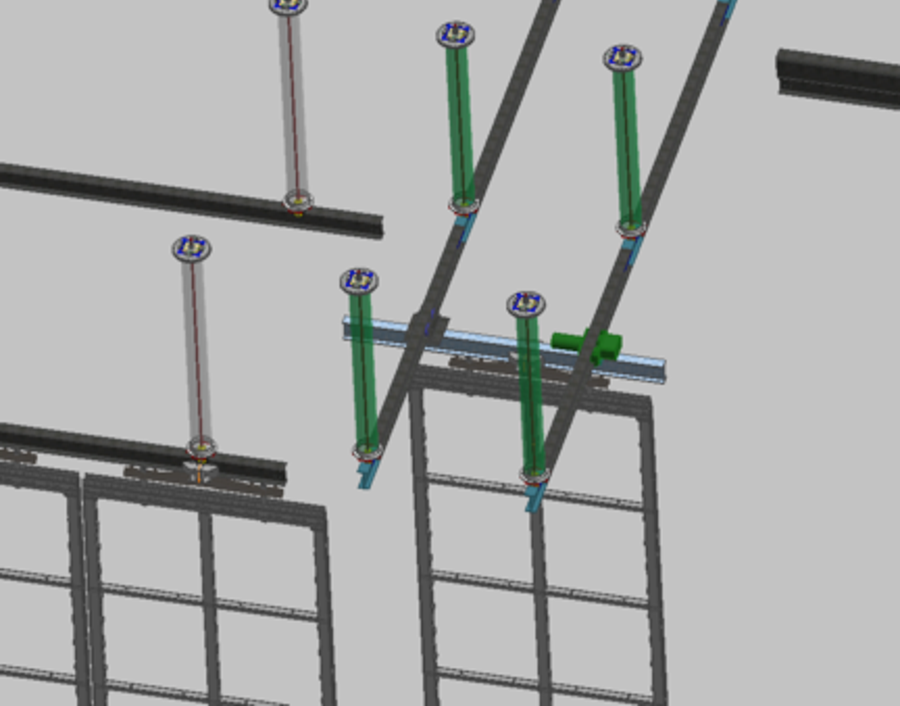
\includegraphics[width=.49\textwidth]{/Shuttle-1.pdf}
 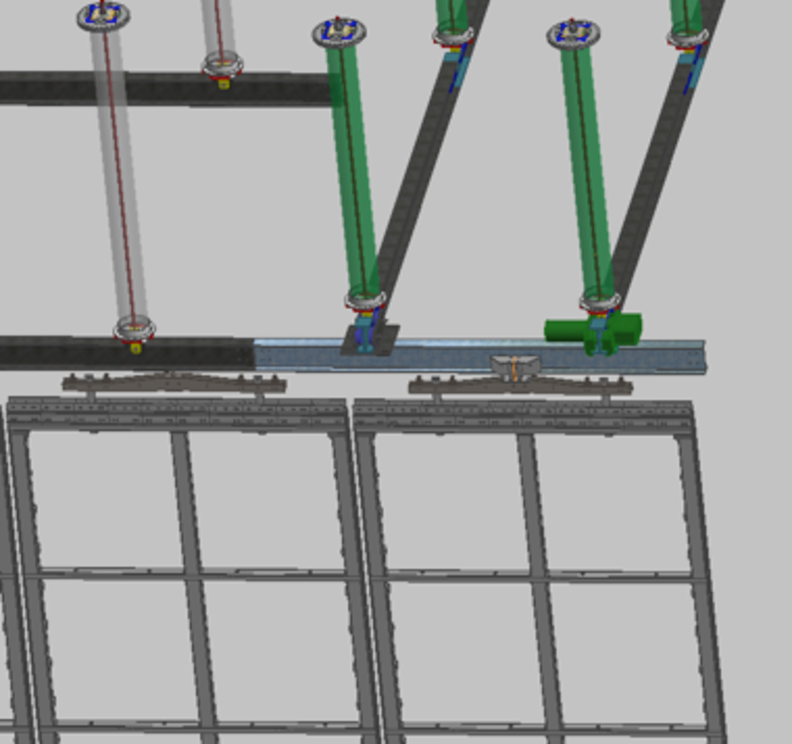
\includegraphics[width=.42\textwidth]{shuttle-2.pdf}
\end{dunefigure}


The \dword{dss} installation begins with the placement and alignment of all
the \fdth{}s onto the flanges that are mounted to the warm vessel.
There are \num{25} \fdth{}s per row and five rows for a total of \num{125}
\fdth{}s.  A fixture with a tooling ball is attached to the
clevis of each \fdth.  The $xy$ position in the horizontal plane
and the vertical $z$ position of this tooling ball is defined, then a %.  A
survey is performed to determine the location of each tooling
ball center and $xy$ and $z$ adjustments are made to get the tooling
ball centers to within $\pm$\SI{3}{mm}.  The \SI{6.4}{m} long I-beams are then 
raised and pinned to the clevis.  Each beam weighs roughly \SI{160}{kg} (\SI{350}{lbs}).
A lifting tripod is placed over each of the \fdth{}s
supporting a beam, and a \SI{0.64}{cm} \SI{0.25}{in}  %$1/4 ^{''}$ 
cable is fed through the top
flange of the \fdth down the \SI{14}{m} to the cryostat floor where it
is attached to the I-beam.  The winches on each tripod raise
the beam in unison in order to get it to the correct height to be
pinned to the \fdth clevis.  Once the beams are mounted, a final
survey of the beams takes place to ensure they are properly located and aligned
to each other.

A mock-up of the shuttle system is constructed to test the
mechanical interlock and drive systems for the shuttle beam
for each \dword{detmodule}.  Tests are conducted to evaluate the level of
misalignment between beams that can be tolerated and the amount of
positional control that can be achieved with the motorized trolley. It
is expected this will be finished prior to the \dword{tdr}. At the time of the
\dword{tdr} a larger prototype installation at Ash River will be under
construction. This prototype will use full scale elements and will be
used to develop the installation procedures and to test the
\dword{detmodule} installation process.
